\documentclass[a4paper,10pt,xelatex,ja=standard,twocolumn]{bxjsarticle}
\usepackage[dvipdfmx]{graphicx}
\usepackage{amsmath}
\usepackage{latexsym}
\usepackage{multirow}
\usepackage{url}
\usepackage{here}
\usepackage{siunitx}
\usepackage{listings}

\lstset{
  language = html,
  backgroundcolor={\color[gray]{.90}},
  breaklines = true,
  breakindent = 10pt,
  basicstyle = \ttfamily\scriptsize,
  frame = TBrl,
  framesep = 2pt,
}

\title{麻婆豆腐のおいしい作り方}
\author{kat0h}
\date{\today}

\begin{document}

\maketitle

おいしい麻婆豆腐を家庭で作りたかった記録。

\begin{figure}[h]
  \caption{麻婆豆腐}
  \label{mapo_top}
  \begin{center}
    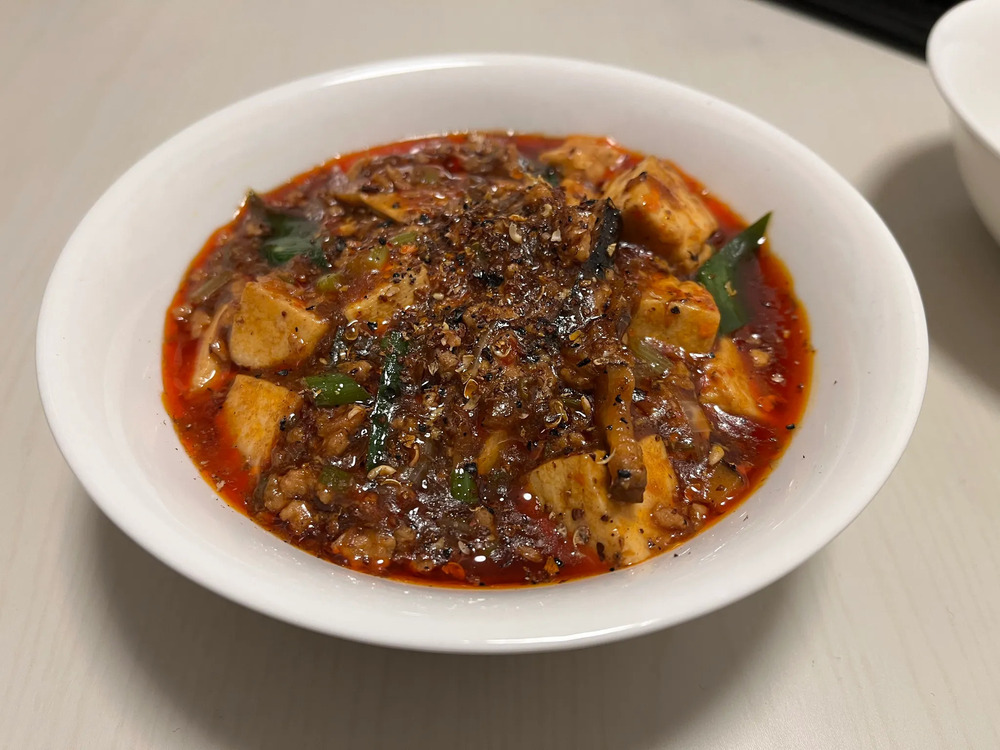
\includegraphics[width=\linewidth]{IMG_3694.jpg}
  \end{center}
\end{figure}


\section{麻婆豆腐とは}

麻婆豆腐は、中国・四川省発祥の料理で、豆板醤を使った辛みのあるスープに豆腐を加えて煮立たせたものである。1862年にに四川省の料理人に、陳劉氏によって考案されたもので、比較的歴史が浅い。\cite{1}

日本で広まった四川式の麻婆豆腐のレシピは四川飯店の創業者である陳建民によって伝えられたものがベースになっている。さらに、日本では中国政府公認の「陳麻婆豆腐店」が2000年から営業しており、本場のレシピで提供している。\\

\section{材料}

麻婆豆腐の基本的な材料は以下の通りである。以降の章では特に重要な材料と、調理道具などについて説明する。

\begin{itemize}
  \item 豆板醤
  \item 甜麺醤
  \item 豆鼓
  \item 花椒
  \item 粉唐辛子
  \item 生姜
  \item ニンニク
  \item 木綿豆腐
  \item 挽肉
  \item 葱
  \item 中華スープ
  \item 辣油
  \item 砂糖
\end{itemize}

\section{豆板醤}

麻婆豆腐の味の決め手は豆板醤である。
私は郫県豆板醤(図\ref{tobanjan})を使っている。郫県豆板醤は中国の郫県(ピーシェン)で作られている豆板醤で、長期間熟成されることが特徴である。長期間熟成されることで、通常の豆板醤よりも色が黒くなり旨味がでる。
郫県豆板醤は通常の豆板醤よりも固く色が出にくいため、あらかじめ少量の水と油で炒めておくことにした。油で炒めることで赤い色がでて、香りも開く。
通常の豆板醤よりも辛さのトゲが少ないが量を増やすと塩気も増えてしまうため、辛さの調節には粉唐辛子を増やすとよい。


\begin{figure}[h]
  \caption{郫県豆板醤 \cite{2}}
  \label{tobanjan}
  \begin{center}
    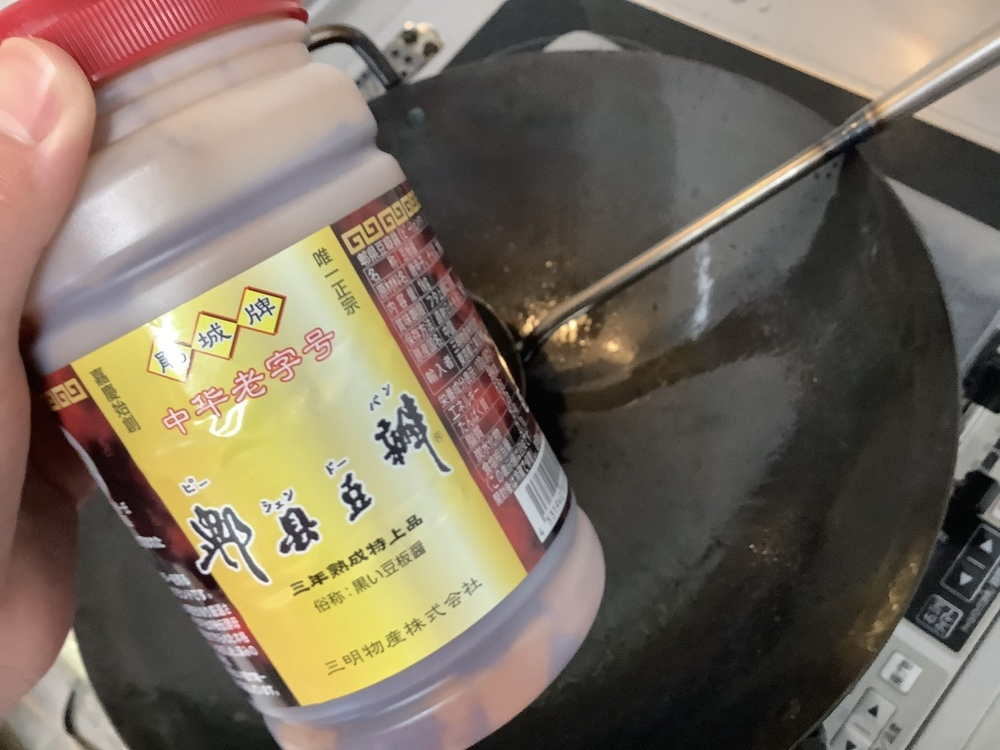
\includegraphics[width=\linewidth]{IMG_4092.jpg}
  \end{center}
\end{figure}

\section{豆腐}

豆腐には木綿豆腐を使う。絹漉し豆腐の方が口溶けが良いが、崩れやすく調理の難易度が高い。
1.5cm程度の賽の目状に切り沸騰した湯で下茹でする。

\section{豆鼓}

豆鼓は黒大豆を発酵させた納豆に近い食材である。独特の香りを持つが、炒めることでとても良い旨味となる。
スーパーなどでは豆鼓を刻み油などと炒めたものが豆鼓醤として販売されている。

\begin{figure}[h]
  \caption{使用した豆鼓}
  \label{tochi}
  \begin{center}
    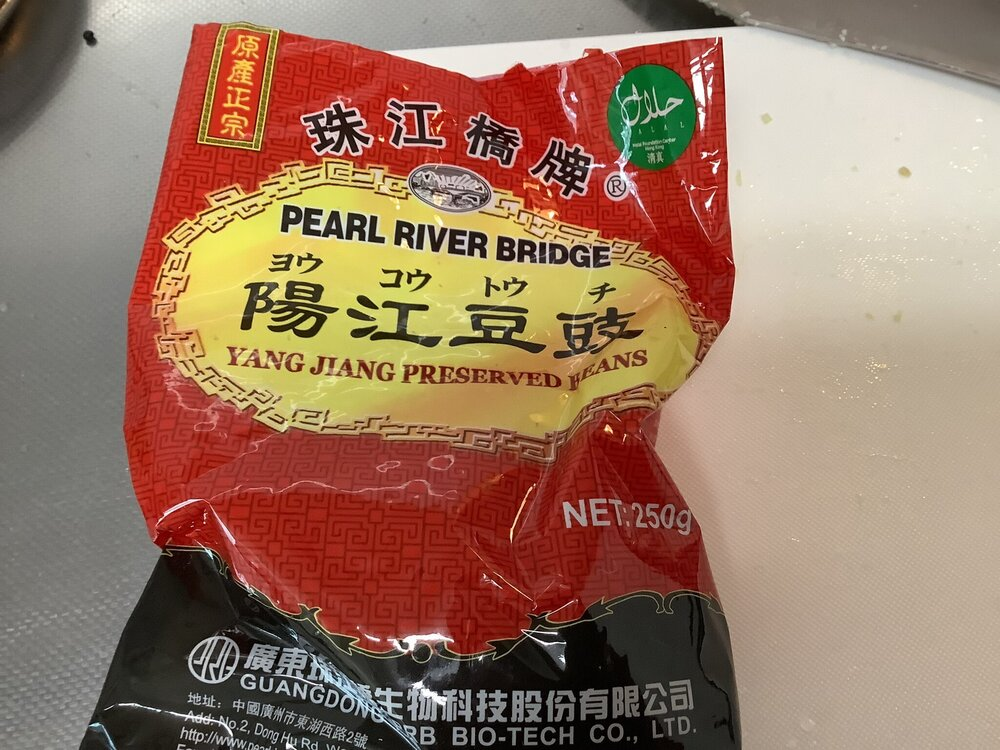
\includegraphics[width=\linewidth]{IMG_4091.jpg}
  \end{center}
\end{figure}

\section{辣油}

辛さを足すだけでなく、仕上りの見た目を良くするために辣油を使用する。スーパーなどで販売されている小瓶の辣油を使っても良いが、すぐなくなる上、高いので自作することにした\cite{3}。
自作にはサラダ油・粉唐辛子・唐辛子・葱・花椒・生姜・八角を使用する(図\ref{rayu})。

\begin{figure}[h]
  \caption{辣油の材料}
  \label{rayu}
  \begin{center}
    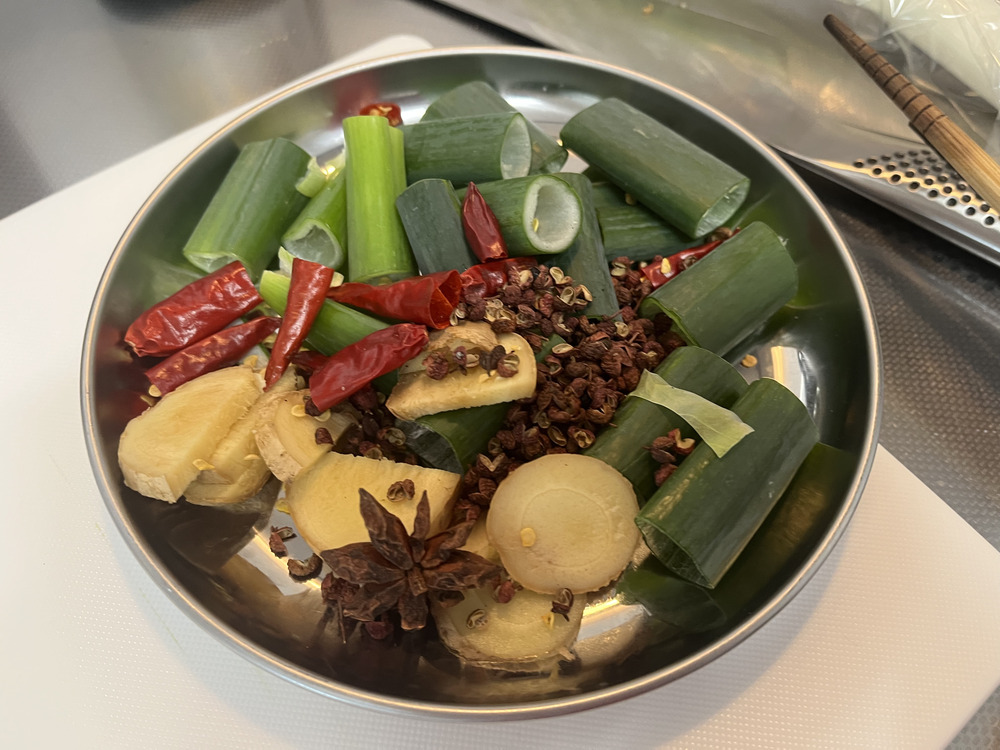
\includegraphics[width=\linewidth]{IMG_4078.jpg}
  \end{center}
\end{figure}

用意した材料を油とともに鍋で加熱した後、葱などから香りが十分に移ったら油を漉し、少量の水で練った粉唐辛子に油を熱いままかけて作る。

\begin{figure}[h]
  \caption{香りを移している様子}
  \label{rayu2}
  \begin{center}
    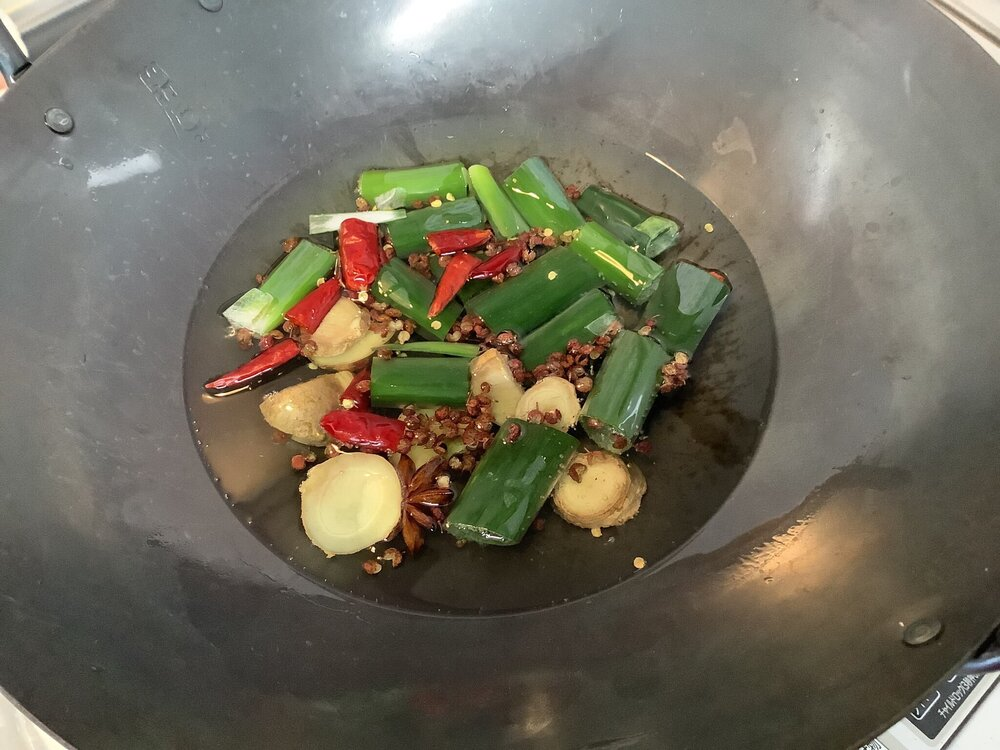
\includegraphics[width=\linewidth]{IMG_4094.jpg}
  \end{center}
\end{figure}

\begin{figure}[h]
  \caption{完成した辣油}
  \label{rayu3}
  \begin{center}
    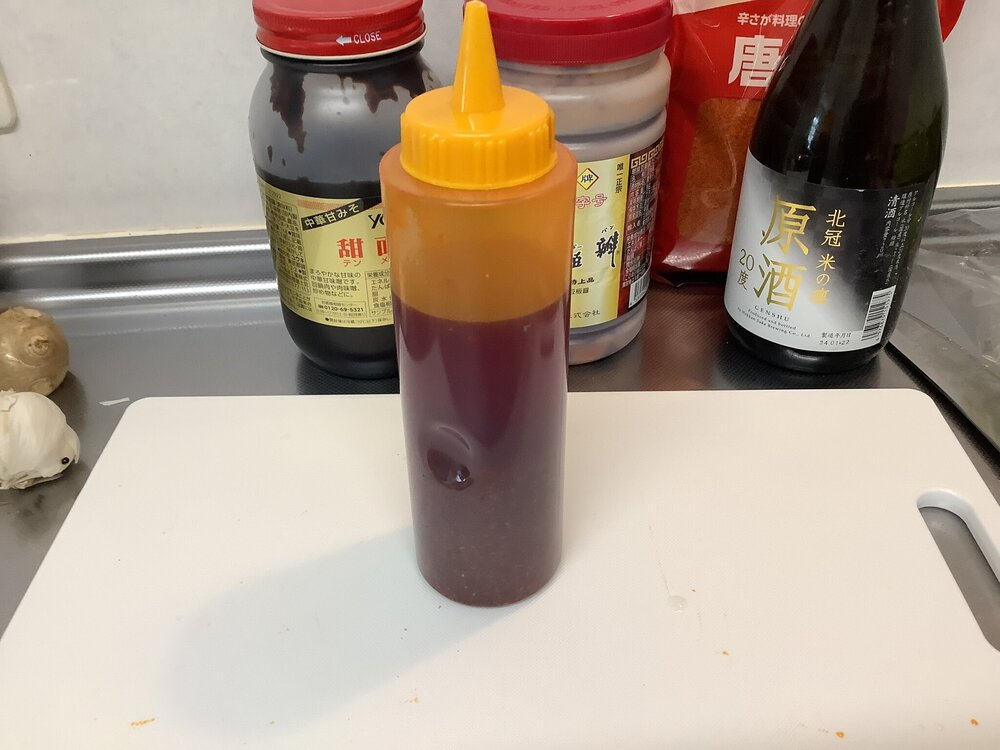
\includegraphics[width=\linewidth]{IMG_4090.jpg}
  \end{center}
\end{figure}

\section{調理道具}

中華料理の厨房で使われている機材を揃えると、より楽に美味しく作れる。なにより楽しい。
自炊として料理を作るのではなく、趣味として作ると長続きすると思う。

\subsection{中華鍋}

豆板醤や豆鼓など材料を炒めるために底の丸い鍋があるとやりやすい。一箇所に液体が集まるためである。

そもそも中華鍋がなぜあの形をしているのかを考察する。
中華料理は大火力のバーナーで食材に一気に火を通し短時間で料理を仕上げるという特徴を持つ。
油が多いのというのも油を熱を伝える媒体として利用して火を素早く通すためだと考えられる。
よって、鍋は火の熱を即座に食材に伝えられるものでなくてはならない。また、高温に耐えられる必要もある。

\begin{figure}[h]
  \caption{広東鍋を空焚きしている様子}
  \label{nabe1}
  \begin{center}
    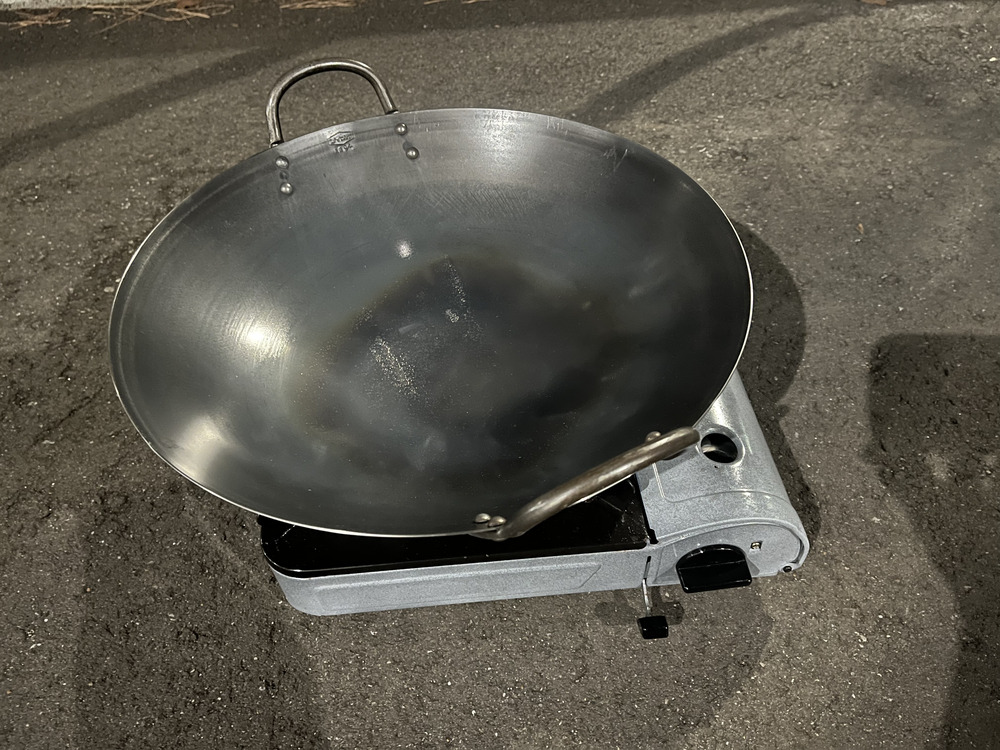
\includegraphics[width=\linewidth]{IMG_3828.jpg}
  \end{center}
\end{figure}

中華鍋には大きく北京鍋と広東鍋がある。北京鍋は底が深い片手鍋で、広東鍋は比較的底が浅い両手鍋である。
基本的にどちらの鍋を使うかは好みだが、北京鍋は重心が片方に寄っているため炒め物には持ちやすく便利な反面、煮物には不安定なため不向きである。

自宅では30cmと36cmの広東鍋を購入した。鉄板の厚さは1.2mmで火にかけるとすぐ表面まで熱が回る。チタニウムなどの素材は熱伝導率が低すぎるため焦げ付きやすく、アルミニウムは柔らかく熱に弱いので薄い鍋には不向きである。

大抵の料理は36cmの鍋でこなす。家庭で使うには少々大きいが、多少振っても材料が溢れないため麻婆豆腐の調理にはとても便利である。
小回りが効くサイズとして30cm、オールラウンダーなサイズとして36cmと使い分けた。

山田工業所が作っている中華鍋が国内で購入できる中では一番上等なものである。浅草近くの河童橋道具街で複数の店が販売している。おすすめの店を下に示すので参考にしてほしい。

\begin{itemize}
  \item 釜浅商店: 新しい建物で器具を選ぶ楽しさがある。個人客をターゲットにしているのか、店員さんがとても親切で分からないことなども教えてくれるはず。(\url{https://kama-asa.co.jp/} )
  \item 藤田道具: 500円ほど相場より鍋が安いらしい。(\url{https://fujitadougu.com/})
  \item ヤマヤ: 山田工業所の鍋が常時複数あるかも。(\url{http://yamaya-s.co.jp})
  \item 銅源サイトウ: すこし分厚い1.6mmの鍋の取り扱いあり。(\url{http://www.dougen-saito.co.jp/})
\end{itemize}

自宅の36cm鍋は中尾アルミ製作所のものを使っている。既に中華鍋の製造を辞めてしまったようだが、河童橋に直営店が複数あるほかデッドストック品が安価に出回っている可能性がある。

\begin{figure}[h]
  \caption{河童橋道具街のシンボル}
  \label{nabe1}
  \begin{center}
    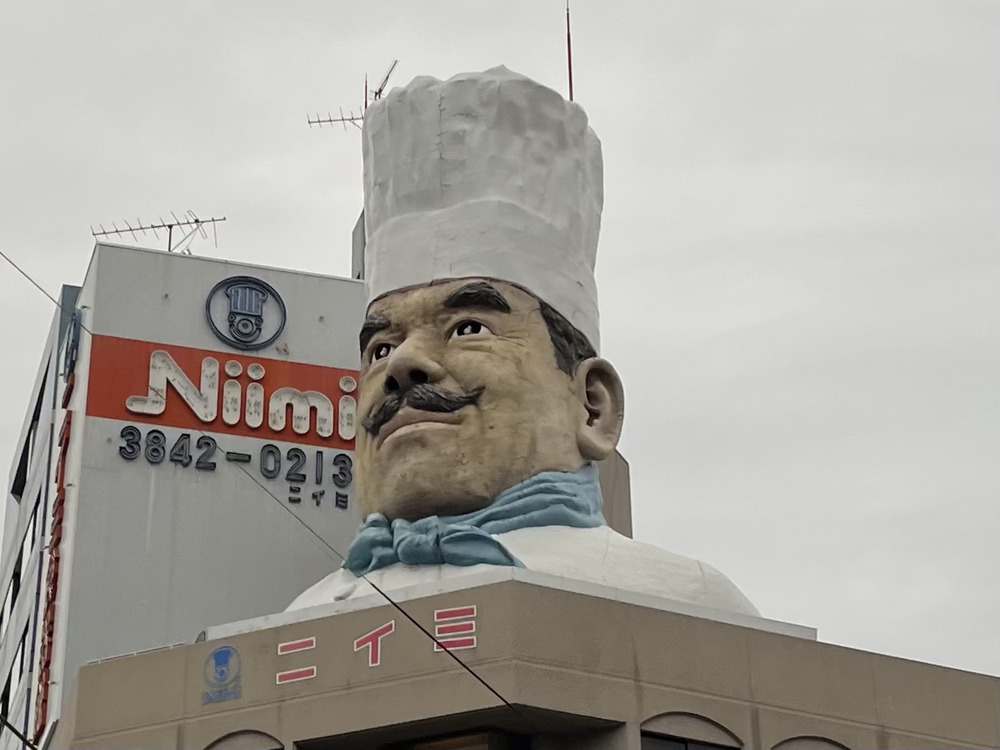
\includegraphics[width=\linewidth]{IMG_4014.jpg}
  \end{center}
\end{figure}

\subsection{おたま}

中華鍋を購入するならセットで買いたいのが鉄もしくはステンレスで作られたお玉である。
おたま一つで掬う・混ぜる・計量する・延すなど多彩な動作をすることができる。
200mlサイズのおたまが36cmなべに丁度良く、1cupを簡単に計量できるためお勧めする。

\subsection{炸鏈}

炸鏈は片手鍋に多数の穴を空けた形状をしている。スープや油から大きいものを掬い出すのに使われる。
基本的に必需品ではないが鍋から豆腐を掬い上げたり、油淋鶏を作るときに肉に油を掛けたりするために非常に便利な道具である。

\begin{figure}[h]
  \caption{炸鏈}
  \label{jaren}
  \begin{center}
    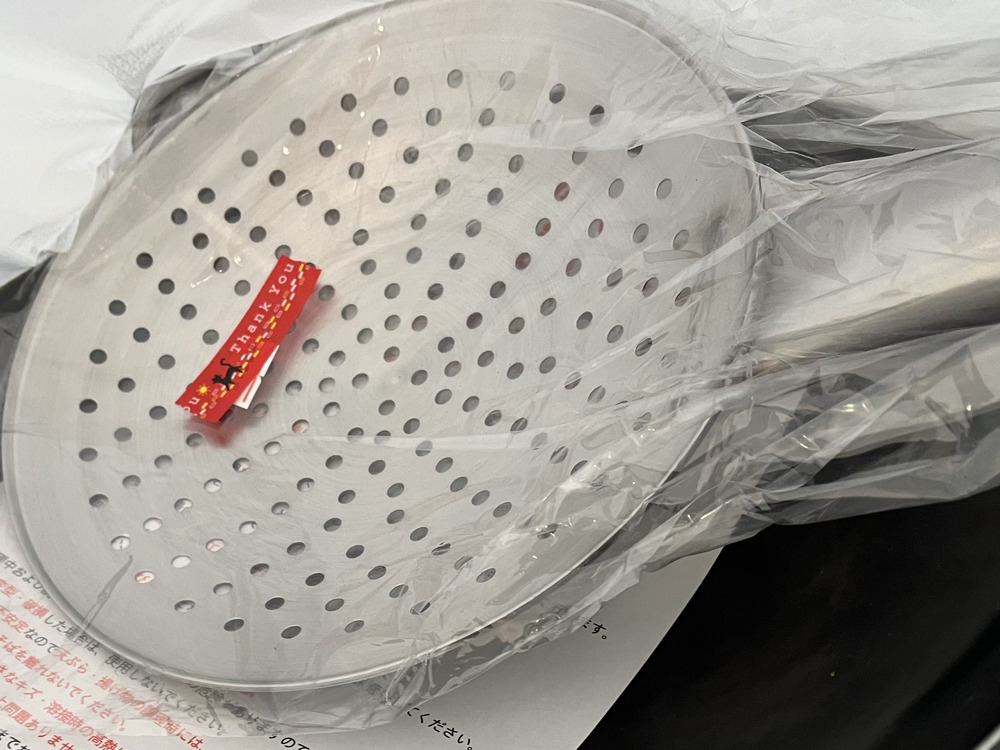
\includegraphics[width=\linewidth]{IMG_4016.jpg}
  \end{center}
\end{figure}

\subsection{ステンレスの平皿}

切った材料を載せる、火を通した食材を一度上げる、落し蓋にするなど様々な用途で使用できる。
ステンレスだと雑に扱えるほか、薄く収納できる。調理器具として買うと一枚300円~と少々値が張るが、100円ショップでキャンプグッズとして販売されているものだと模様があるが安い。4枚あれば大抵の料理には不自由しない。

\begin{figure}[h]
  \caption{使用している平皿}
  \label{jaren}
  \begin{center}
    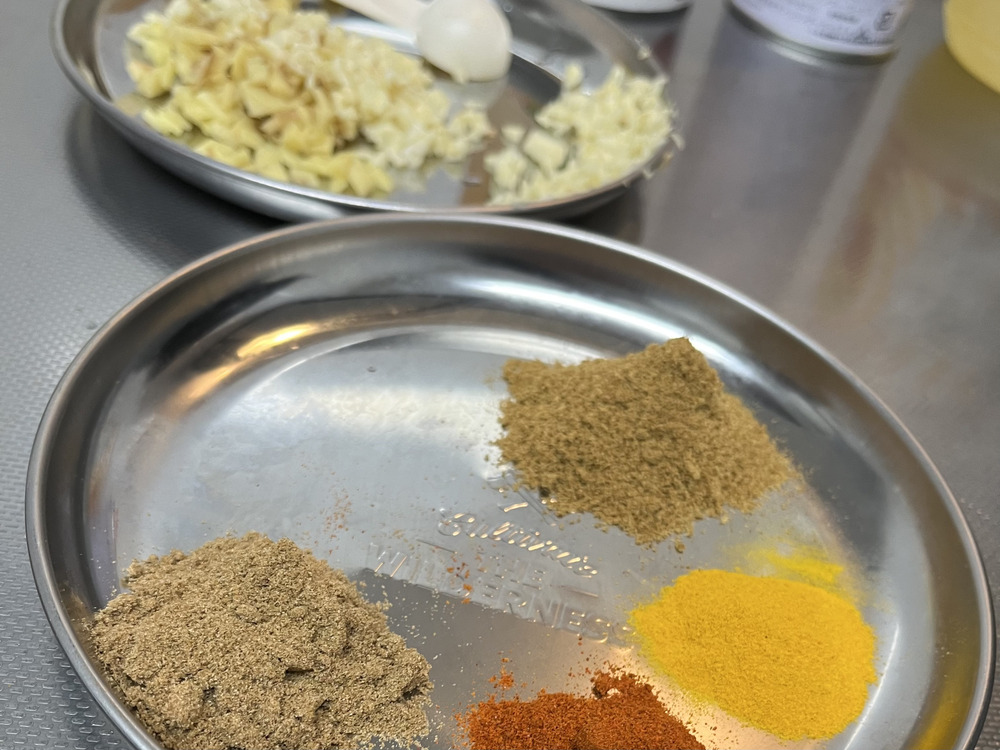
\includegraphics[width=\linewidth]{IMG_3985.jpg}
  \end{center}
\end{figure}

\section{調理工程}

\begin{figure}[h]
  \caption{材料の準備}
  \label{ziaryo}
  \begin{center}
    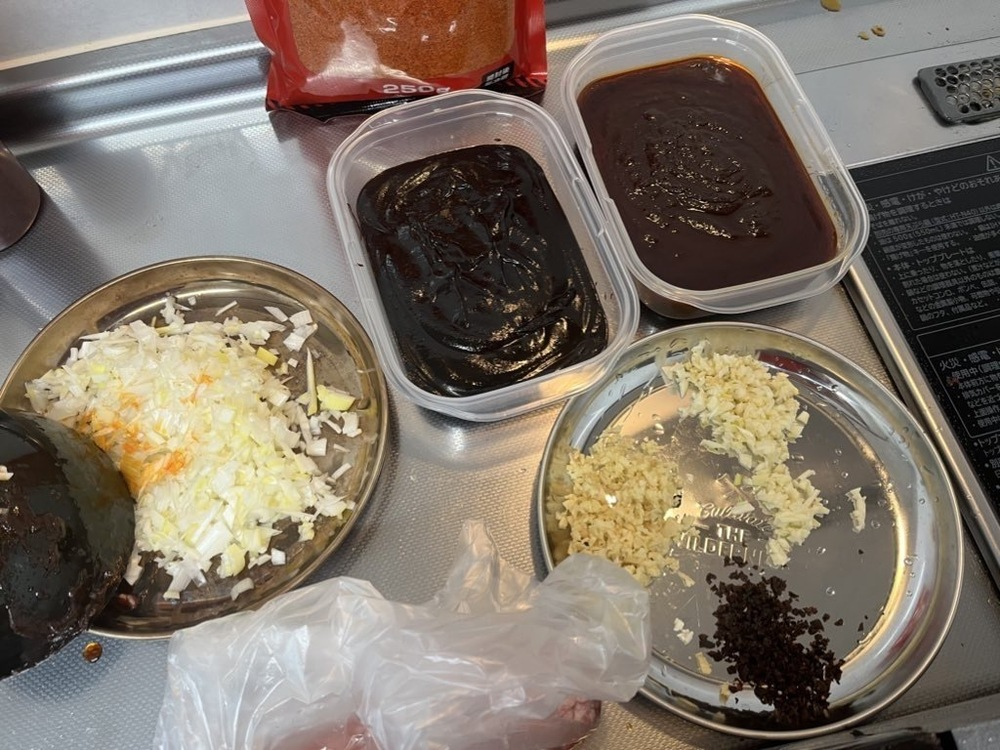
\includegraphics[width=\linewidth]{IMG_4080.jpg}
  \end{center}
\end{figure}

\subsection{挽肉を炒める}

本来の麻婆豆腐は牛挽肉を利用するが高価で入手性が悪いため、豚挽肉を油を敷いた鍋で炒める。
ここで重要なのが、挽肉をしっかり炒めることである。豚肉は特有の臭みを持つが、火を良く通すことで臭みを消すことができる。
初め挽肉は白く濁った色の油を出すが、臭みが飛ぶころになると透明な油になる。

また、肉が焦げる寸前までしっかり火を通すことで食感を出す。酥と表現され、サクサクした食感にすることが重要である。

火を通したら、甜麺醤を絡ませ軽く炒める。甜麺醤は焦げやすいため、軽く炒めるだけで良い。
できた味付きの肉は一度別皿に取っておく。

\begin{figure}[h]
  \caption{肉を炒めている様子}
  \label{niku}
  \begin{center}
    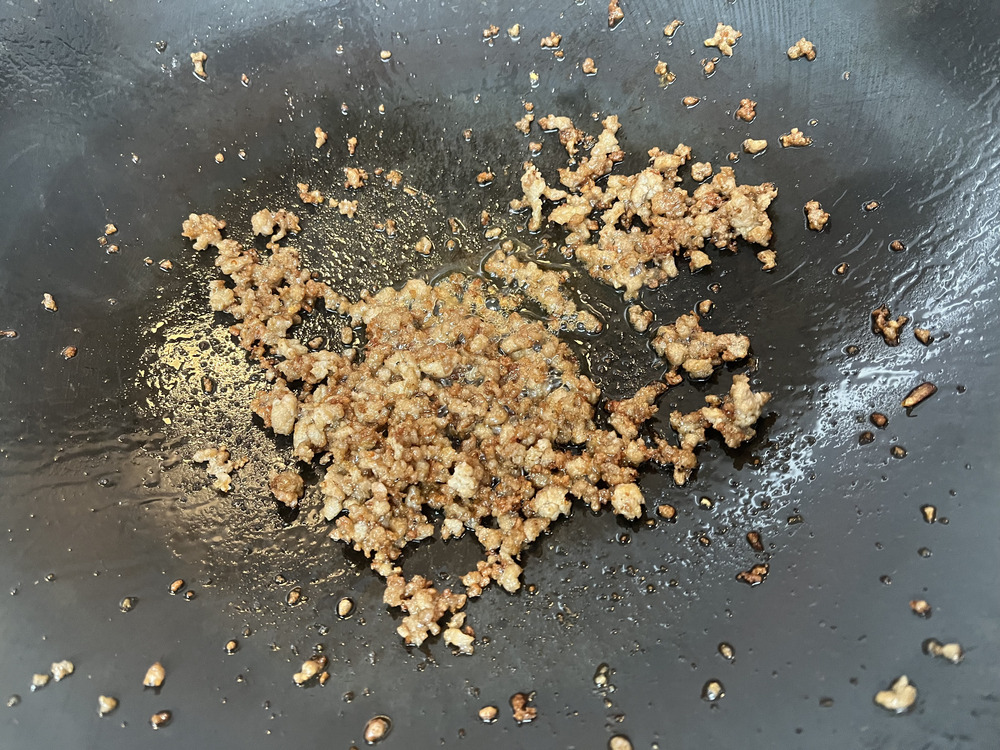
\includegraphics[width=\linewidth]{IMG_4081.jpg}
  \end{center}
\end{figure}

\subsection{スープを作る}

鍋に油を多めに敷き、みじん切りにした生姜とにんにくを香りが出るまで炒める(焦がさないように注意)。
十分に香りが出たら豆板醤と好みの量の粉唐辛子を加え、表面に無数の泡が湧き立つ程度炒めて油に豆板醤の赤みを移す。赤みを移せるタイミングは今しかないため、しっかりと炒めること。

豆鼓を加えたら鶏ガラスープを350ccほど入れる。スープは顆粒のものを使用しても良いし、味覇などのスープの素を使っても良い。
表面に赤い油が出てきたところで、酒・醤油・砂糖を少量加える。

\begin{figure}[h]
  \caption{できたスープ}
  \label{tofu}
  \begin{center}
    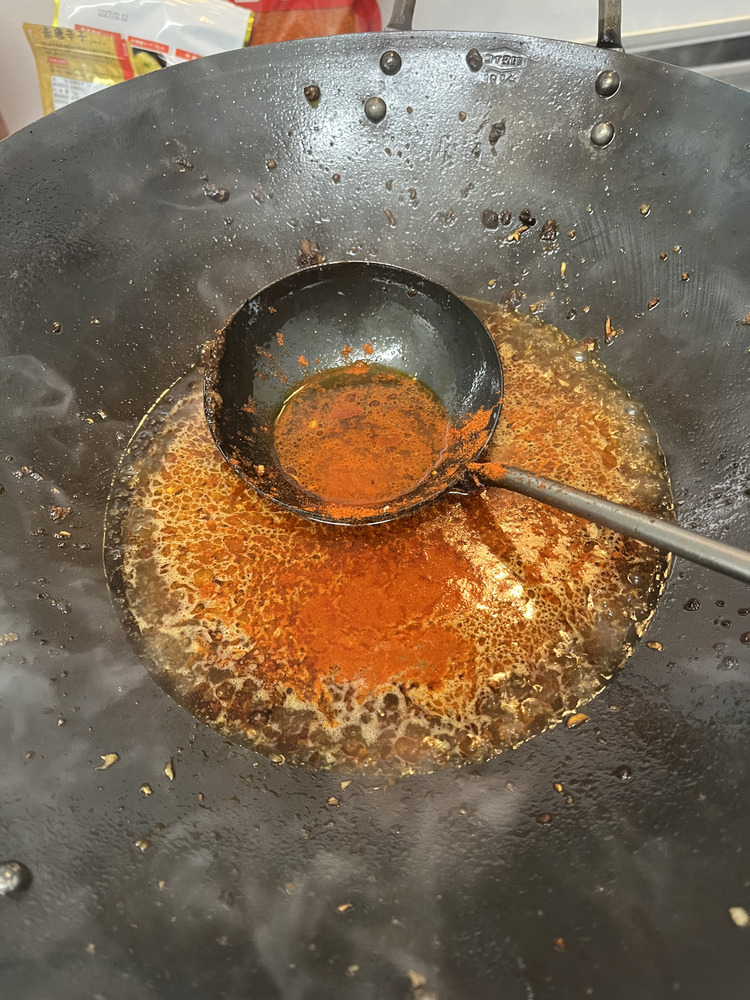
\includegraphics[height=\linewidth]{IMG_4082.jpg}
  \end{center}
\end{figure}

\subsection{豆腐を茹でる}

鍋に少量の塩を入れた湯を沸かせる。沸騰した湯に賽の目にした豆腐を入れ、再度沸騰したあたりで豆腐を引き上げる。

\begin{figure}[h]
  \caption{下茹でした豆腐}
  \label{tofu}
  \begin{center}
    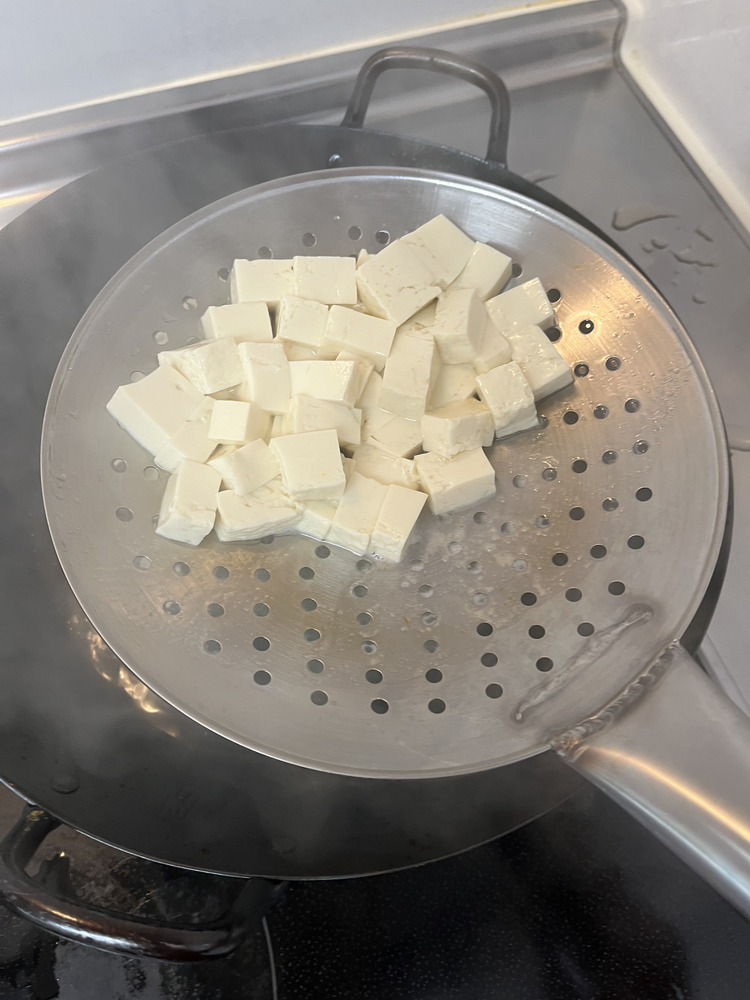
\includegraphics[height=\linewidth]{IMG_4085.jpg}
  \end{center}
\end{figure}

\subsection{煮込む}

豆腐を煮込む。このとき、おたまで豆腐を崩さないように注意する。
基本的に混ぜる際はおたまの丸い面で豆腐を押すようにする。別の角度から混ぜるときは鍋を回して中の角度を変えるようにする。

1分ほどたったらみじん切りにしておいた葱を混ぜる。このあたりからスープの流動性が低くなる。

\begin{figure}[h]
  \caption{豆腐を煮込んで味を付ける}
  \label{tofu}
  \begin{center}
    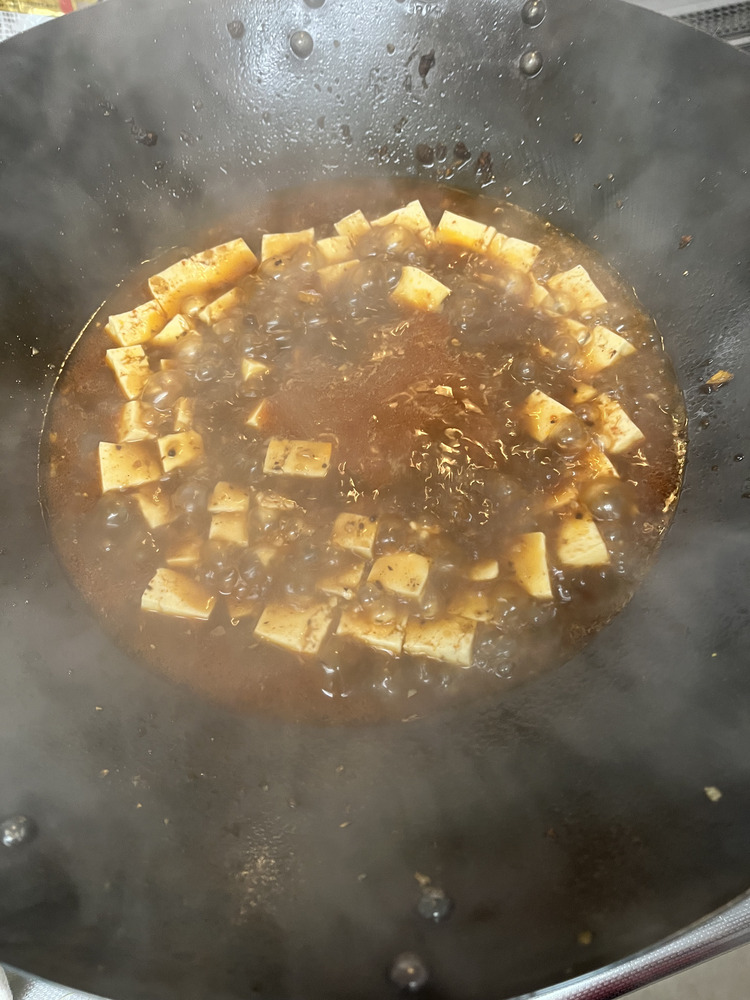
\includegraphics[height=\linewidth]{IMG_4086.jpg}
  \end{center}
\end{figure}

\subsection{固める}

おたまで押したとき道ができる程度に固まったら、別にしておいた肉を全体に馴染ませる。
水解き片栗粉を回し入れ、かき混ぜる。このとき強火にしていると片栗粉がすぐに固まってしまい、うまくとろみがつかないため注意する。

全体に行き渡ったら辣油を表面に掛ける。この辣油は飾り油として機能する。
最後に香りを出しつつ、片栗粉を固めるために強火で加熱する。片栗粉は加熱しないととろみを出さない。

\begin{figure}[h]
  \caption{とろみを付けた様子}
  \label{tofu4}
  \begin{center}
    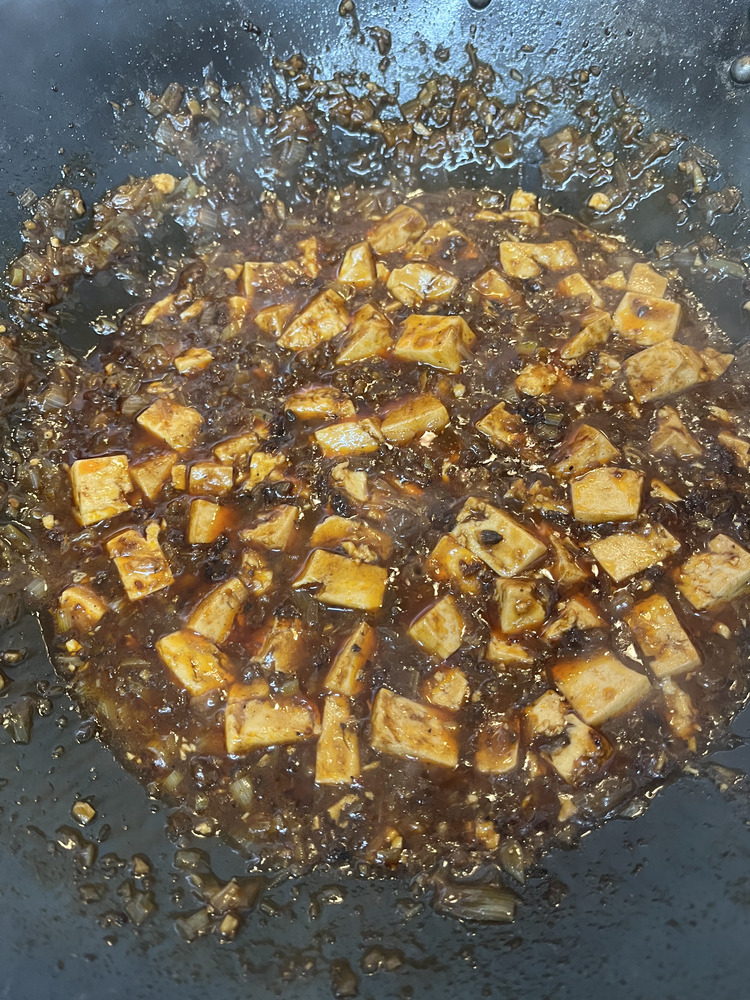
\includegraphics[height=\linewidth]{IMG_4087.jpg}
  \end{center}
\end{figure}

\subsection{もりつけ}

器に盛り付けたら、細かく挽いた花椒を掛ける。麻婆豆腐で重要な味わいの、麻辣の麻の部分となる。

\begin{figure}[h]
  \caption{完成品}
  \label{final}
  \begin{center}
    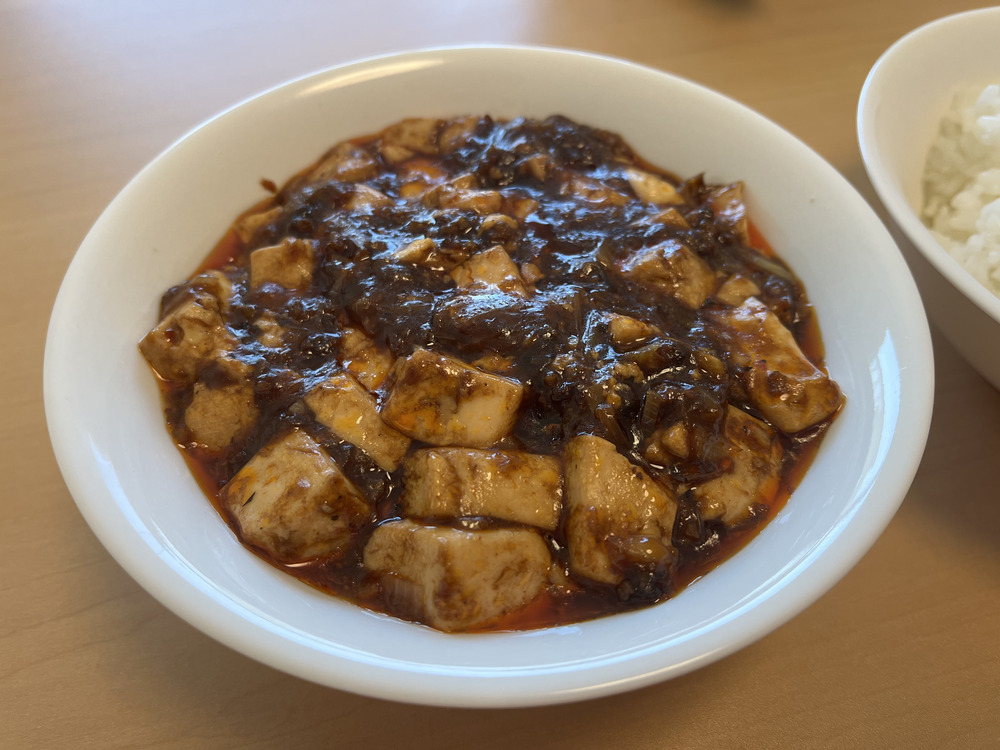
\includegraphics[width=\linewidth]{IMG_4089.jpg}
  \end{center}
\end{figure}

\section{おわりに}

陳健一のレシピを基に、調理するなかで気づいたことなどをまとめました。
麻婆豆腐は簡単に調理できる上、味も安定しやすい便利な料理です。
ぜひ、麻婆豆腐を作ってみて欲しいです。

\section{参考文献}
\begin{thebibliography}{99}
\bibitem{1} 麻婆豆腐発祥の店「陳麻婆豆腐」のストーリー, \url{https://chenmapo.jp/history/}
\bibitem{2} 三明物産 郫県豆瓣, \url{https://sannmei.co.jp/product/%e9%83%ab%e7%9c%8c%e8%b1%86%e7%93%a3%e9%86%a4%e3%83%94%e3%83%bc%e3%82%b7%e3%82%a7%e3%83%b3%e3%83%88%e3%82%a6%e3%83%90%e3%83%b3%e3%82%b8%e3%83%a3%e3%83%b3/}
\bibitem{3} ホットペッパーグルメ 自家製ラー油の作り方を「四川料理のスゴイ人」に教わってきた, \url{https://www.hotpepper.jp/mesitsu/entry/noriki-washiya/19-00089}
% \bibitem{2} 伝統的な麻婆豆腐を構成する八か条 \url{https://chenmapo.jp/tradition}
\bibitem{4} とにかく売れたい中華屋, 【有料級】10年かかって覚えた技を10分で教える人。, \url{https://www.youtube.com/watch?v=Zc5QlyB8s2c}
\bibitem{5} 料理王国, 陳建一 シェフ 「究極の麻婆豆腐」|赤坂四川飯店, \url{https://www.youtube.com/watch?v=VbZxN0sKuVg&t=602s}
\end{thebibliography}

\end{document}



